\documentclass[14pt,xcolor=dvipsnames, handout]{beamer}% version imprimable avec notes d’orateur, handout
\usepackage[couleur]{/home/basile/Git/Latex/Headfiles/dipneuste}
%\usepackage[couleur]{/home/basile/Latex/Headfiles/dipneuste}
%\usepackage[orientation=portrait,size=A4]{beamerposter}
\usepackage{pgfpages}
\uselanguage{French}
\languagepath{French}
\usetheme{Madrid}
% See http://goo.gl/Wxlyy for alternative themes
 
% Specify base color
\usecolortheme[named=OliveGreen]{structure}
%\usefonttheme[onlymath]{serif}
%\mode<beamer>{\usetheme{Darmstadt}%}
\setbeamercolor{math text}{fg=DarkBlue}%
\setbeamercolor{math text displayed}{fg=DarkBlue}
%\setbeameroption{show notes on second screen = right}
\setbeameroption{show only notes}
\pgfpagesuselayout{2 on 1}[a4paper,border shrink=5mm]
\title{Cohomologie des figures impossibles}
\author{Basile Pillet}
\date{}

\newcommand<>{\pleinecran}[2]{{
    \setbeamertemplate{navigation symbols}{}
    \newgeometry{margin=0pt}
    \begin{frame}
    \includegraphics[width=\paperwidth]{#1}
    \note{#2}
    \end{frame}
    }
}
%\AtBeginSection{
    %\begin{frame}[c,plain,noframenumbering]
        %\tableofcontents[currentsection,hideothersubsections]
    %\end{frame}
%}

\newcommand\vis[1]{\fbox{\textcolor{DarkGreen}{#1}}}
\newcommand*{\vcenteredhbox}[1]{\begingroup
\setbox0=\hbox{#1}\parbox{\wd0}{\box0}\endgroup}


%\setbeamertemplate{note page}[plain]
\setbeamertemplate{navigation symbols}{}



%\newcommand{\nota}{\note}
\newcommand{\nota}[1]{\note{\begingroup \quad {#1}\par \bigskip\endgroup}}
%\AtBeginNote{$\bullet$\quad }

\begin{document}

\begin{frame}
  \maketitle
  \vspace*{-3em}
\begin{center}
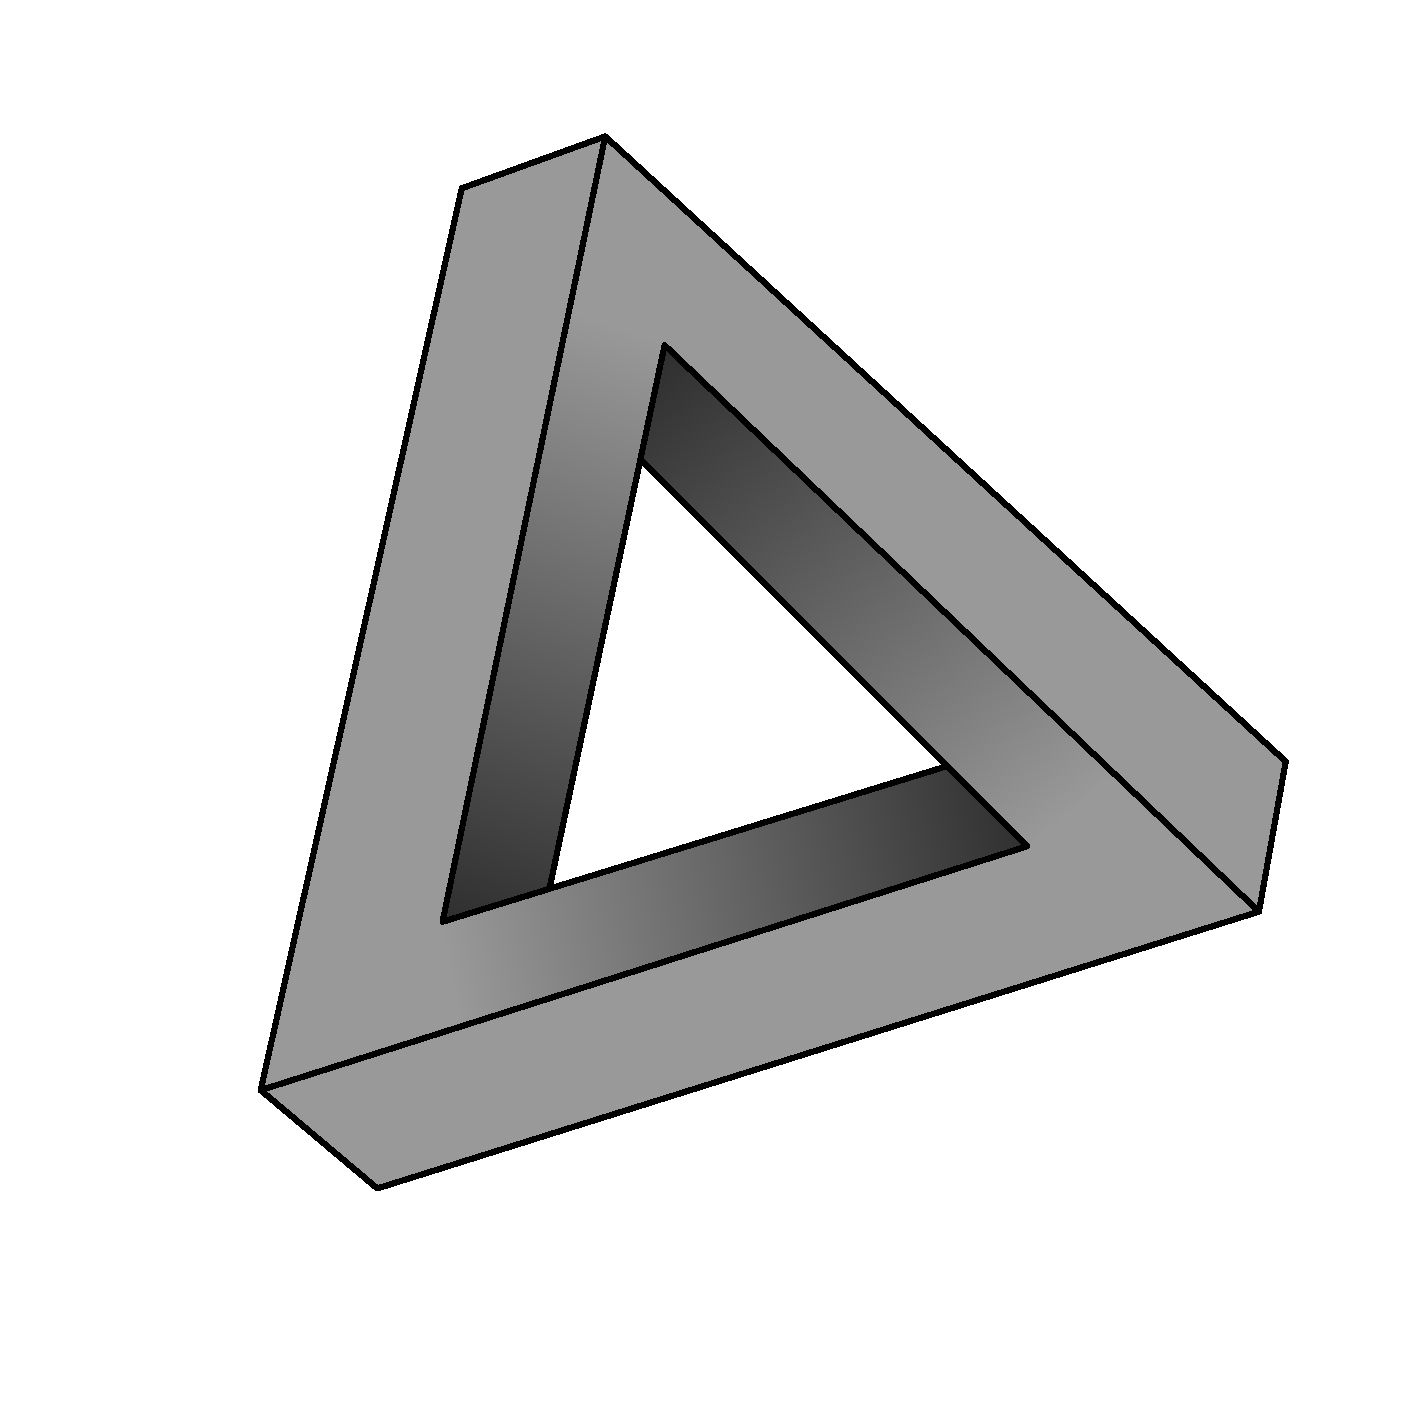
\includegraphics[scale=.25]{../Images/tribar_ombre.pdf}
\end{center}
\nota{Bonjour, je m'appelle Basile Pillet et je suis doctorant à l'institut de mathématiques de Rennes. Je vais vous parler d'un outil d'algèbre et de géométrie qu'on appelle \textit{Cohomologie} et je vais vous le présenter sur l'exemple du \textit{triangle de Penrose}.}
\nota{Le \textit{triangle de Penrose}, c'est l'objet impossible dessiné ici.}
% Il a été créé par le physicien et mathématicien Sir Roger Penrose dans les années 50. Il a alors été présenté comme étant "\textit{L'impossibilité dans sa forme la plus pure}".}
\nota{On va se servir de la cohomologie pour identifier ce qui empêche un tel objet d'exister.}
\end{frame}


\newgeometry{margin=0pt}

\begin{frame}% POSSIBLE LOCALEMENT
\begin{center}
\nota{On part de notre objet impossible}
\includegraphics<1|handout:0>[scale=.4]{../Images/tribar.pdf}
\nota{Si on ne regarde que le coin en haut à gauche ...}
\includegraphics<2>[scale=.4]{../Images/UpperCorner.pdf}
\nota{... on remarque qu'il n'a plus rien d'impossible !}
\includegraphics<3|handout:0>[scale=.4]{../Images/UpperCorner2.pdf}
\nota{On peut le réaliser en vrai avec deux bouts de bois et un peu de colle}
\includegraphics<4|handout:0>[scale=.4]{../Images/UpperCorner3.pdf}
\end{center}
\end{frame}


\begin{frame}% Recouvrement
\begin{center}
\nota{Revenons à notre \textit{triangle de Penrose} ou plutôt son dessin}
\includegraphics<1|handout:0>[scale=.4]{../Images/tribar.pdf}
\nota{On peut découper ce dessin en trois parties autour de chaque coin.}
\includegraphics<2|handout:0>[scale=.4]{../Images/Covering.pdf}
\nota{...parties qui s'intersectent suivant la zone en rouge}
\includegraphics<3>[scale=.4]{../Images/Covering2.pdf}
\end{center}
\end{frame}


\begin{frame}% Split
\begin{center}
\nota{Éclatons donc notre dessin. On a trois dessins qui chacun représente des objets RÉALISABLES}
\includegraphics<1>[scale=.4]{../Images/Covering_split.pdf}
\nota{Ces trois dessins doivent être recollés suivant les zones rouges pour obtenir le dessin d'origine.}
\nota{Notre figure impossible est LOCALEMENT possible. Mais si les trois dessins peuvent se recoller pour donner le dessin du \textit{triangle de Penrose}, les trois objets physiques eux ne peuvent pas ! }
\end{center}
\end{frame}


\begin{frame}% Notations
\begin{center}
\nota{Numérotons ces trois parties qui recouvrent le dessin. Prenons un point $A$ à l'intersection de l'objet $1$ et de l'objet $2$}
\includegraphics<1|handout:0>[scale=.4]{../Images/A.pdf}
\nota{Après découpage, le point $A$ se dédouble : une copie $A_{1}$ dans $U_1$ et une copie $A_{2}$ dans $U_2$}
\includegraphics<2>[scale=.4]{../Images/Ai.pdf}
\end{center}
\end{frame}


\begin{frame}% Distance observateur
\begin{center}
\nota{
Si maintenant on construit un coin numéro $1$, il aura une certain taille. Et pour qu'il apparaisse tel quel sur le dessin, il faut le mettre à une certaine distance de l'observateur. Si on l'avait construit plus petit, il aurait fallu le mettre plus près.
}
\includegraphics<1>[scale=.5]{../Images/DistanceObservateur2.pdf}
\nota{
Mais le coin numéro $2$ n'est pas forcément à la même distance de l'observateur. Imaginez que l'on construise l'objet $1$ immense mais très loin et l'objet $2$ petit mais très près.
}
\includegraphics<2|handout:0>[scale=.4]{../Images/1Loin2Pres_.pdf}
\end{center}
\end{frame}


\begin{frame}% Dij
\nota{
Pour garder cette information en mémoire, on va noter $d_{12}$ le rapport des distances entre ces deux points.
}
\begin{equation*}
d_{12} = \alt<2>{\dfrac{OA_1}{OA_2}}{\dfrac{\text{ distance du point représenté par }A_{1}\text{ à l'observateur}}{\text{ distance du point représenté par }A_{2}\text{ à l'observateur}}}
\end{equation*}
\end{frame}

\begin{frame}% 6 points
\begin{center}
\nota{
On recommence avec un point $B$ sur l'intersection de $U_1$ et $U_3$ et un point $C$ sur l'intersection de $U_2$ et $U_3$
}
\includegraphics<1>[scale=.4]{../Images/6points.pdf}
\end{center}
\end{frame}

\begin{frame}% Dij
\begin{center}
\begin{equation*}
d_{12} = \dfrac{OA_1}{OA_2}
\end{equation*}
\nota{On définit de même entre l'objet $1$ et l'objet $3$ le rapport $d_{31}$}\pause
\begin{equation*}
d_{31} = \dfrac{OB_{3}}{OB_{1}}
\end{equation*}
\nota{et le rapport $d_{23}$}\pause
\begin{equation*}
d_{23} = \dfrac{OC_{2}}{OC_{3}}
\end{equation*}
\end{center}
\end{frame}


\begin{frame}% Recollement
\begin{center}
\frametitle{\hfill Recollement}
\nota{À quelle(s) condition(s) les trois objets construits se recollent-t-ils ?}
Pour se recoller \\
\pause
\bigskip
il faut \nota{Il faut}
\medskip
\begin{itemize}[<+->]
\item que $A_1$ et $A_2$ se superposent\nota{que $A_1$ et $A_2$ se superposent }%
\uncover<5->{ : \quad  $d_{12} = 1$} \nota{Mais si $A_1$ et $A_2$ se superposent ... ils sont à la même distance de l'observateur... donc que le rapport $d_{12}$ vaut $1$.}
\item que $B_1$ et $B_3$ se superposent\uncover<6->{ :  \quad  $d_{31} = 1$}
\item que $C_2$ et $C_3$ se superposent\uncover<7->{ :  \quad  $d_{23} = 1$}
\end{itemize}
\end{center}
\end{frame}


\section{Homothétie}

\begin{frame}% Homothétie
\begin{center}
\nota{Que voyons-nous ?}
\includegraphics<1|handout:0>[scale=.4]{../Images/ABC.pdf}
\includegraphics<2>[scale=.4]{../Images/d12d23d31.pdf}
\nota{C'est l'information importante sur cette construction. Qui ne se voit pas sur le dessin}
\only<3>{Les $d_{ij}$ forment un \textbf{cocycle}.}
\end{center}
\end{frame}

\begin{frame}% Homothétie 2
\begin{center}
\only<1>{\parbox{.7\textwidth}{\large Que se passe-t-il si on multiplie toutes les dimensions de l'objet $1$ ainsi que sa distance à l'observateur, par $\lambda_1 \in \R^{+*}$ ?}}
\nota{Rien ne change}
\includegraphics<2>[scale=.4]{../Images/ABC.pdf}
\end{center}
\end{frame}


\begin{frame}% Homothétie 2
\begin{center}
\nota{Cependant}
\begin{align*}
d_{12} & \mapsto \uncover<2->{\lambda_1 d_{12}} \\[2em]
d_{31} & \mapsto \uncover<3->{\dfrac{d_{31}}{\lambda_1}} \\[2em]
d_{23} & \mapsto \uncover<4->{d_{23}}
\end{align*}
\end{center}
\end{frame}



\begin{frame}% Homothétie 2
  \frametitle{\hfill Recollement 2}
\nota{}
\begin{center}
Il existe une manière de redimensionner les trois objets telle que 
\[
d_{12} = d_{23}= d_{31}  = 1
\] 
%\pause
%( c'est-à-dire de recoller les trois coins en un vrai \textit{triangle de Penrose} )\\
\bigskip
si et seulement si\\
\bigskip\pause
\begin{equation*}
d_{12} = \dfrac{\lambda_1}{\lambda_2} \quad , \qquad d_{31} = \dfrac{\lambda_3}{\lambda_1} \quad  , \qquad d_{23} = \dfrac{\lambda_2}{\lambda_3}
\end{equation*}
\pause
\bigskip
on dit alors que les $d_{ij}$ forment un \textbf{cobord}.
\end{center}
\end{frame}


\begin{frame}
  \frametitle{\hfill Le \textit{triangle de Penrose} existe \\
    \hfill ssi\\
    \hfill les $d_{ij}$ forment un cobord}
  \nota{Donc le \textit{triangle de Penrose} existe si et seulement si les $d_{ij}$ forment un cobord.}
  \pause
\begin{center}
Si c'est le cas alors
\[
d_{12} \times d_{23} \times d_{31}= \pause
\dfrac{\lambda_1}{\lambda_2} \times \dfrac{\lambda_2}{\lambda_3} \times  \dfrac{\lambda_3}{\lambda_1}= \pause
1
\]
\end{center}
\end{frame}

\section{Contradiction}
\begin{frame}
  \frametitle{\hfill Contradiction}
\nota{On va montrer que c'est absurde}
\begin{center}
\begin{align*}
1 &= d_{12} \times d_{23} \times d_{31}\\
\uncover<2->{&= \dfrac{OA_1}{OA_2} \times \dfrac{OC_2}{OC_3} \times \dfrac{OB_3}{OB_1}\\}
\uncover<3->{&= \dfrac{OA_1}{OB_1} \times \dfrac{OC_2}{OA_2} \times \dfrac{OB_3}{OC_3}}
\end{align*}
\end{center}
\nota{En revenant à la définition, on écrit chaque $d_{ij}$ comme un rapport de distances}
\nota{On peut réorganiser ce produit en un produit de $3$ termes qui ne dépendent chaque que d'un seul objet.}
\end{frame}

\begin{frame}% 1
\nota{Concentrons nous sur l'objet $1$, la perspective nous dit que le point $A_1$ est plus proche de l'observateur que le point $B_1$}
\begin{tikzpicture}
    \node[inner sep=0] (image1) at (0,0) {%
    				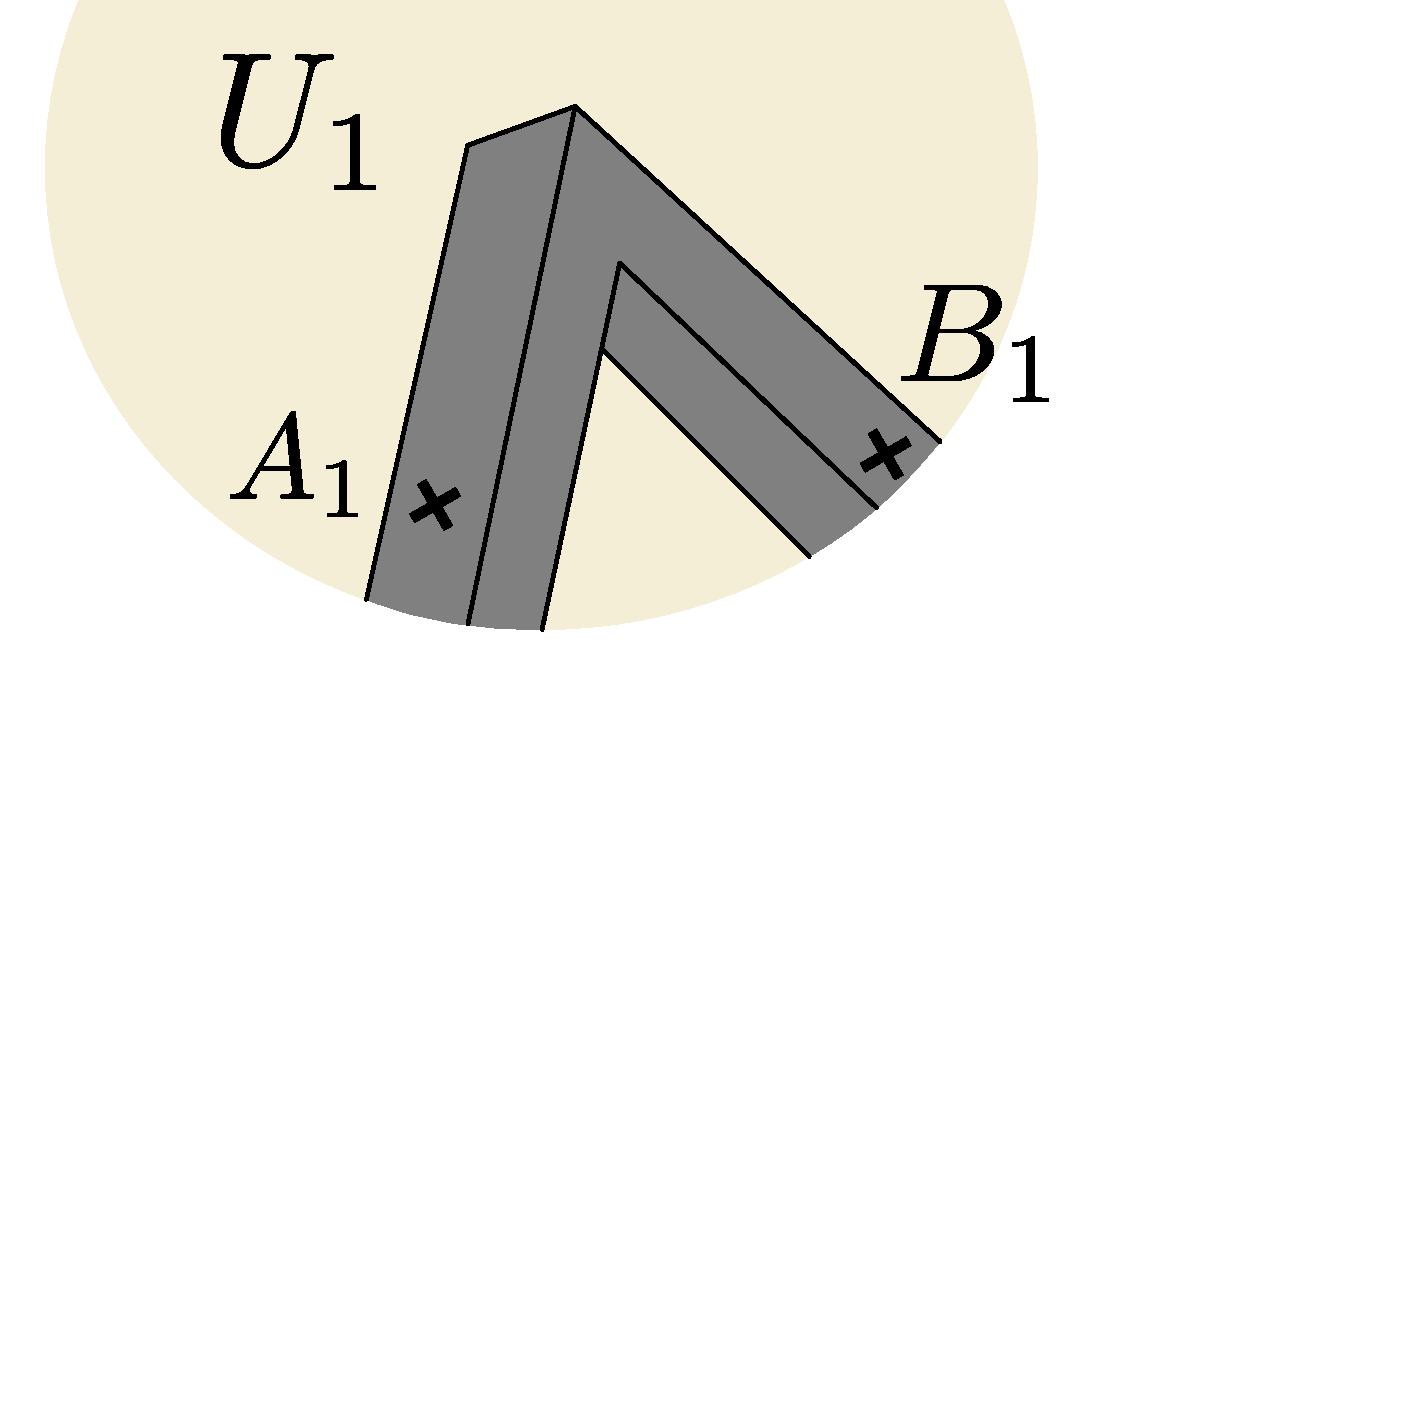
\includegraphics[scale=.4]{../Images/A1<B1.pdf}%
    				};
	\node<2> (AB) at (3,-2) {\LARGE $\displaystyle OA_{1} < OB_{1}$};
	\node<3> (ABbis) at (3,-2) {\LARGE $\displaystyle \dfrac{OA_{1}}{OB_{1}} < 1$};
\nota{Donc le rapport $OA_1/OB_1$ est inférieur à $1$}
\end{tikzpicture}
\end{frame}

\begin{frame}
  \frametitle{\hfill Contradiction}
\begin{center}
\begin{align*}
1 &= d_{12} \times d_{23} \times d_{31}\\
&= \dfrac{OA_1}{OA_2} \times \dfrac{OC_2}{OC_3} \times \dfrac{OB_3}{OB_1}\\
&= \underset{<1}{\underbrace{\dfrac{OA_1}{OB_1}}} \times \dfrac{OC_2}{OA_2} \times \dfrac{OB_3}{OC_3}\\
\end{align*}
\end{center}
\end{frame}

\begin{frame}% 2
\nota{De même pour l'objet $2$, le point $C_2$ apparaît plus proche que le point $A_2$}
\begin{tikzpicture}
    \node[inner sep=0] (image2) at (0,0) {%
    			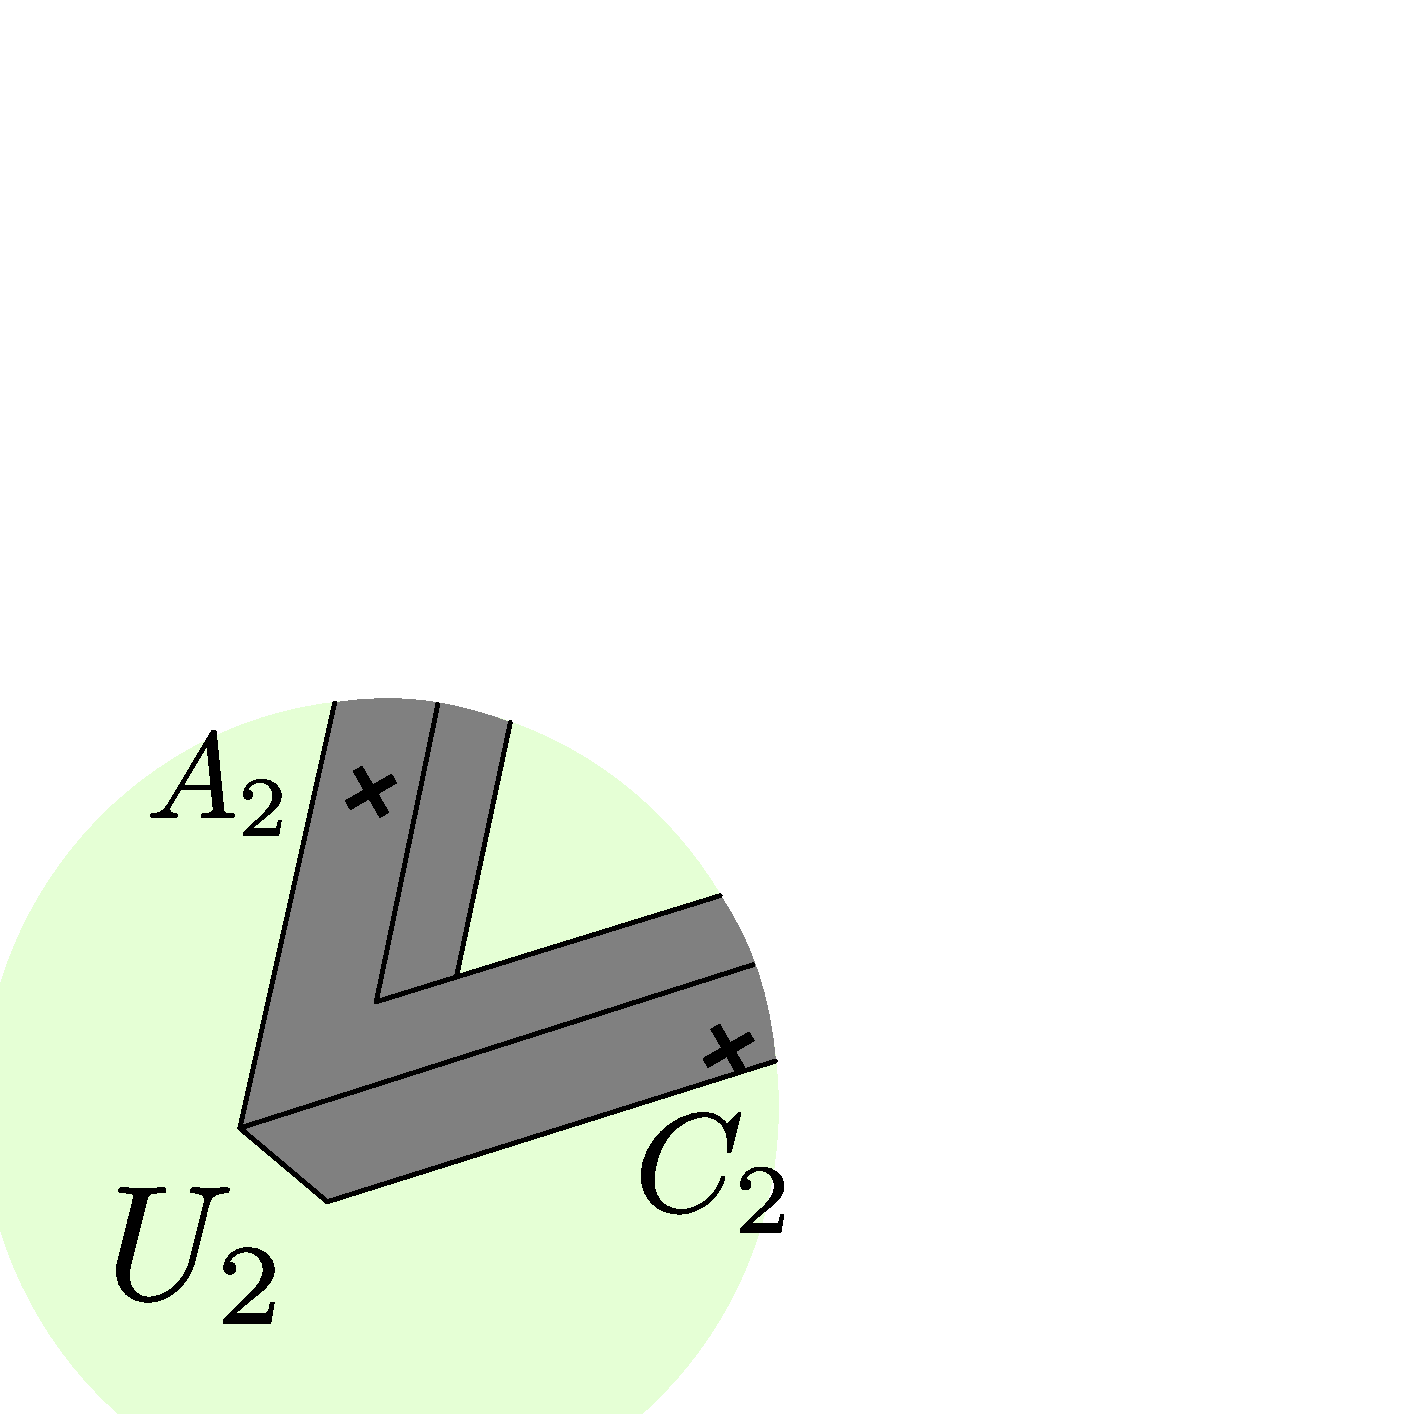
\includegraphics[scale=.4]{../Images/A2>C2.pdf}%
    			};
	\node<2> (CA) at (3,2) {\LARGE $\displaystyle OC_{2} < OA_{2}$};
\end{tikzpicture}
\end{frame}


\begin{frame}
  \frametitle{\hfill Contradiction}
\begin{center}
\begin{align*}
1 &= d_{12} \times d_{23} \times d_{31}\\
&= \dfrac{OA_1}{OA_2} \times \dfrac{OC_2}{OC_3} \times \dfrac{OB_3}{OB_1}\\
&= \underset{<1}{\underbrace{\dfrac{OA_1}{OB_1}}} \times \underset{<1}{\underbrace{\dfrac{OC_2}{OA_2}}} \times \dfrac{OB_3}{OC_3}\\
\end{align*}
\end{center}
\end{frame}


\begin{frame}% 3
\nota{De même pour l'objet $3$, le point $B_3$ apparaît plus proche que le point $C_3$}
\begin{tikzpicture}
    \node[inner sep=0] (image3) at (0,0) {%
    			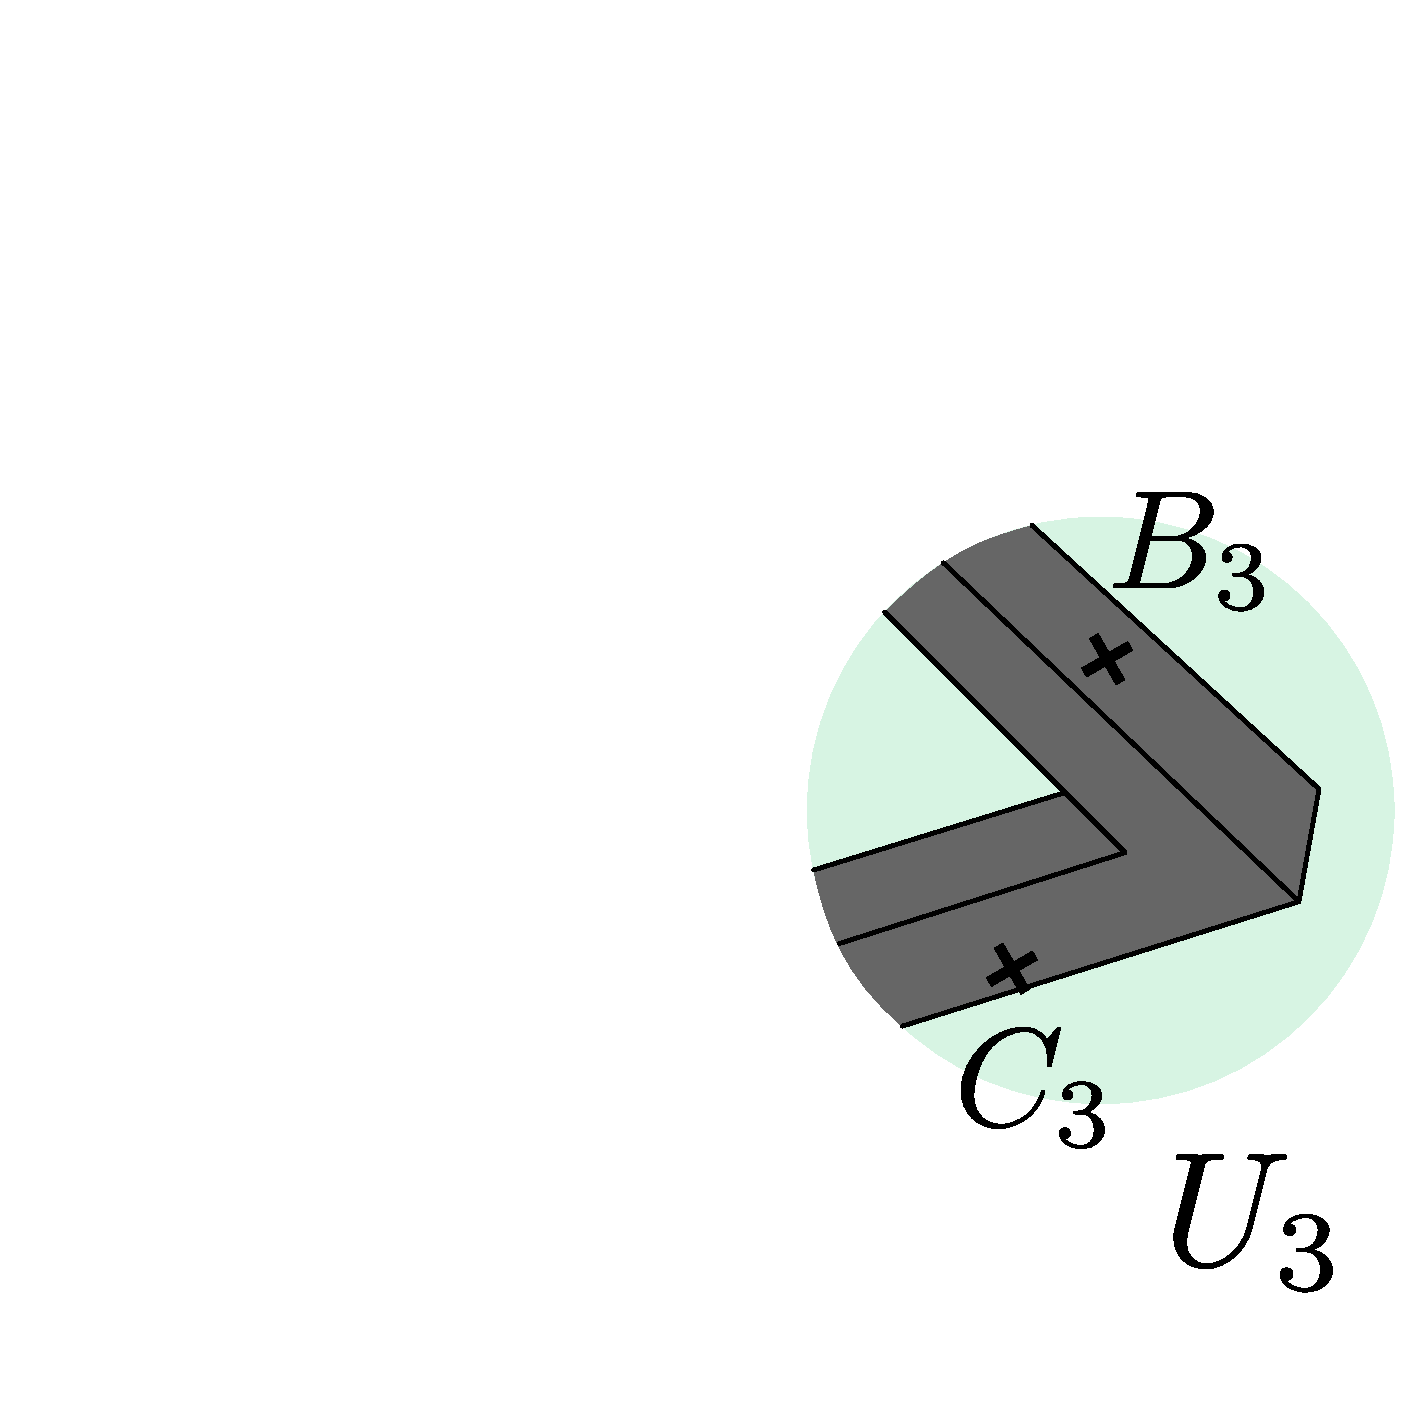
\includegraphics[scale=.4]{../Images/B3<C3.pdf}%
    			};
	\node<2> (BC) at (-2,3) {\LARGE $\displaystyle OB_{3} < OC_{3}$};
\end{tikzpicture}
\end{frame}


\begin{frame}
  \frametitle{\hfill Contradiction}
\begin{center}
\begin{align*}
1 &= d_{12} \times d_{23} \times d_{31}\\
&= \dfrac{OA_1}{OA_2} \times \dfrac{OC_2}{OC_3} \times \dfrac{OB_3}{OB_1}\\
&= \underset{<1}{\underbrace{\dfrac{OA_1}{OB_1}}} \times \underset{<1}{\underbrace{\dfrac{OC_2}{OA_2}}} \times  \underset{<1}{\underbrace{\dfrac{OB_3}{OC_3}}}\\
\uncover<2->{&< 1}
\end{align*}
\nota{Finalement chacun des trois rapports est strictement inférieur à $1$, on a donc une contradiction}
\uncover<3->{Le \textit{triangle de Penrose} n'existe pas.}
\nota{Le \textit{triangle de Penrose} n'existe pas.}
\end{center}
\end{frame}

\begin{frame}
\begin{center}
\nota{L'intérêt n'est pas de montrer que le \textit{triangle de Penrose} est impossible ! L'intérêt c'est qu'en mathématique (en algèbre et en géométrie), quand quelque chose ne marche pas, eh bien la vie ne s'arrête pas. Il y a \textbf{des choses}, de nouveaux objets, qui empêchent que ça marche et l'étude de ces \textbf{obstructions} se révèle bien souvent très riche}\vspace*{-2.5em}
\hspace*{-6em}\includegraphics<1>[scale=.87]{../Images/lego-triangle.jpg}
\end{center}
\end{frame}

\end{document}
